\documentclass[authoryear,preprint,review,10pt]{elsarticle}
\usepackage{amssymb,amsthm,amsmath,setspace}
\usepackage{url,color}
\usepackage{lineno}
%\usepackage[labelfont=bf,format=hang,textfont=it]{caption}
\usepackage{graphicx}
\usepackage{microtype}
\usepackage[letterpaper,text={15cm,23cm}]{geometry}
\usepackage{natbib}
\usepackage{hyperref}

%% for internal use
\newcommand{\fixme}[1]{\emph{\marginpar{FIXME} (#1)}}
\newcommand{\readme}[1]{\emph{\marginpar{README} (#1)}}

\definecolor{Red}{rgb}{0.5,0,0}
\definecolor{Blue}{rgb}{0,0,0.5}
\hypersetup{%
  pdftitle = {Real-time land cover disturbance detection using satellite image time series},
  pdfsubject = {remote sensing, monitoring},
  pdfkeywords = {early warning, real-time, change detection, land cover change, REDD, deforestation, disturbance, NDVI, time series, MODIS, vegetation dynamics, phenology},
  pdfauthor = {Jan Verbesselt, Achim Zeileis, Martin Herold},
  %% change colorlinks to false for pretty printing
  colorlinks = {true},
  linkcolor = {Blue},
  citecolor = {Blue},
  urlcolor = {Red},
  hyperindex = {true},
  linktocpage = {true},
}


\journal{Remote Sensing of Environment}

\begin{document}
%% \linenumbers
\begin{frontmatter}

    \title
    {
    Real-time land cover disturbance detection \\ using satellite image time series \\
%    A case study for early warning of Drought in the Horn of Africa
    %real-time change detection using satellite image time series:
    %Early warning for forest disturbances
    % Real-time change detection of forest disturbances using satellite image time series
    }
    \author[WUR]{Jan Verbesselt\corref{cor}}
    \ead{Jan.Verbesselt@wur.nl}
    \author[UIBK]{Achim Zeileis}
    \ead{Achim.Zeileis@R-project.org}
    \author[WUR]{Martin Herold}
    \ead{Martin.Herold@wur.nl}
    \cortext[cor]{Corresponding author.}
    \address[WUR]{Remote Sensing Team, Wageningen University, \\
           Droevendaalsesteeg 3, Wageningen 6708 PB, The Netherlands}
    \address[UIBK]{Department of Statistics, Universit\"at Innsbruck \\
           Universit\"atsstr.~15, A-6020 Innsbruck, Austria}

\singlespace

\begin{abstract}

% satellite image time series are faster and faster available - methods to deal with this are lacking
Real-time monitoring of land cover disturbances are critical for addressing impacts on carbon storage, biodiversity, and socio-ecological processes. Satellite remote sensing enables cost-effective and accurate monitoring at frequent time steps over large areas. Yet, generic methods to detect disturbances within newly captured satellite images are lacking. 

We propose a generic time series analysis approach to detect disturbances within newly acquired data by automatically identifying a stable history period to model normal expected behaviour and as such enable detection of abnormal change (i.e. disturbances like drought effects, fires or deforestation events).

Time series of vegetation greenness provide evidence of terrestrial vegetation productivity over the last decades covering the whole world and therefore contain essential information related land cover dynamics and disturbances. Here, we assess and demonstrate the method by (1) simulating time series of vegetation greenness data from satellite data with different amount of noise, seasonality and disturbances, (2) applying it to real satellite greenness image time series between February 2000 and July 2011 of the Horn of Africa to  detect drought related vegetation disturbances.

Simulation results illustrate the proof-of-concept of the proposed real-time monitoring method. Disturbances are successfully detected in real-time, i.e., at the end of a time series, while being robust for seasonality and noise. However, the noise level of the time series remains the most important driver of capacity and timeliness to detect changes. As such, data pre-processing in order to improve the quality and reliability of time series data remains essential to improve disturbance detection. 

An homogenous region of drought related anomalies were detected in the South of Somalia illustrating the capacity of the method. Vegetation greenness related disturbances were successfully detected by restricting the analysis to areas with a minimum amount of vegetation cover and by requiring a minimum length of 2 years of the automatically detected stable history period.

The method is publicly available within the \emph{BFAST} package for {R}. This method is developed so that it can be used at a global scale since is fast, does not depend on vegetation type specific thresholds or definitions and does not require gap filling of time series. The method is flexible and can be applied for different purposes (e.g., deforestation, drought or fire or detection) and to different types time series data (e.g., climate data, in-situ monitoring sensors or different biophysical parameters derived from satellite image time series). 


%
%Validation and accuracy assessment of the near real-time change detection method is done by  (1)~simulating 16-day MODIS NDVI time series with different amount of noise, seasonality and containing disturbances with different magnitudes, (2)~using real MODIS satellite image time series of Eastern Africa.

%Results illustrate the proof-of-concept of the proposed real-time monitoring method. Disturbances are successfully detected in real-time, i.e., at the end of a time series, while being robust (?)for seasonality and noise.  % de methode houdt rekening met seasonaliteit maar kan wel seasonal and trend changes detecteren - dus dit klopt ook niet echt.
% onderstaande is ook een zwakke zin want de methode kan overal eigenlijk gebruikt worden...

%Further work is needed for operational implementation of the method to enable a rapid response and alert system by applying it to time series data with a
%high temporal resolution (e.g., hourly or daily data). \\

% further validation is required to verify it capacity to detect specific change types in relation to the type and quality of time series data that is being used.
% the potential of this method has been illustrated for drought detection in Eastern Africa (within a specific vegetation type) - it was shown that was able to identify drought effects with well in advance and could be used as an extra tools on top of other political and social early warning tools.  This paper only demonstrates the potential the method further testing is required in other ecosystems of the world... % e.g. the simulation exercise illustrated that the method works reasonably well in forested ecosystems since they are more stable (easier to model the history period) whereas the grasslands are more unstable by their nature (lots of seasonal shifts and changes in phenology) which makes it more difficult to detect long term disturbances within grasslands.

% it needs to be clarified that this method is only developed and demonstrated as a generic early warning system for satellite data which directly monitors vegetation dynamics using the NDVI index (biomass/dryness related) however the NDVI is has a lot of advantages and disadvantages...

%We are proposing a time series analysis approach to detect disturbances in near real-time within recently captured satellite images by automatically identifying a stable history period to model normal expected behaviour and enable detection of abnormal changes (i.e. disturbances related to abnormal vegetation dynamics). 

\textbf{Research Highlights}
\begin{itemize}
    \item A novel near real-time time series based change detection approach within newly acquired satellite images.
    \item Validation by simulating time series and applying it on real satellite data.
    \item The approach is robust, fast, and flexible to different data sets and does not require gap filling or smoothing.
    \item The is freely available as a function in the \emph{bfast} package for the open-source statistics system {R}.
\end{itemize}

\end{abstract}

\begin{keyword}
Early warning \sep global change \sep land cover disturbance\sep drought \sep NDVI \sep time series \sep MODIS \sep vegetation phenology \sep dynamics
\end{keyword}

\end{frontmatter} 

\section{Introduction}

% could we orient it more towards drought detection - so link it with the SMOS mission and a recent science paper. % the importance of detecting disturbances in real-time? 
% mention drought related problems - NDVI - rainfall link

Real-time land cover disturbance detecting is critical for tracking human-induced and natural disturbances promptly \citep{Asner:2011fa}. Such
information is needed for signalling abnormal developments, quickly raising awareness, and allow for prompt actions to intervene, relief efforts and reduce negative impacts to natural resources, humans, and infrastructure. 

%Real-time remote sensing approaches are already performed for weather monitoring and
%prediction \citep{Ebert:2007tj} (SMOS/MeteoSAT/ClimateDAta), and in case of after-disasters and relief efforts \citep{Tralli:2005ch}. 

Key to approaches looking at land cover disturbances is that many recent change events occur worldwide at unknown locations with unknown change magnitudes. In this sense, remote sensing tools can be in the first instance used to alert when things start to appear \emph{abnormal}. For example, deviations from \emph{normal} land surface phenology, defined as the seasonal variation in vegetated land surface from remote sensing \citep{White2009}, can indicate important changes in forest health \citep{Stone2008,Morisette2009}, carbon status, regional drought effects and even climate change \citep{Cleland2007,Hargrove2009}.

% satellite data and vegetation indices
Satellite sensors are well-suited to provide consistent and frequent measurements over large areas which is appropriate for capturing the effects of many processes that cause disturbances, including physical (e.g. droughts, fires, floods), biogenic (e.g. herbivorous insects and pathogens) and anthropogenic (e.g. deforestation, urbanisation, farming) disturbances \citep{Jin2005, Potter2003}. A common way to derive indicators of environmental change is the use of spectral vegetation indices such as the Normalised Difference Vegetation Index (NDVI) that is strongly related to the photosynthetic capacity of vegetation canopies \citep{Myneni1995, Pettorelli:2005ed}. % fraction of photosynthetic active radiation (wavelength $0.4-0.7 \mu m$)

% different change types in ecosystem dynamics
Many types of ecosystem changes affecting the land surface range from diurnal cycles to long-term change in vegetation patterns. The ecosystem changes commonly observed with remote sensing approaches can be divided into three categories: (1)~\emph{seasonal or cyclic change}, driven by annual temperature and rainfall interactions impacting plant phenology resulting in distinct intra-annual patterns for different vegetation types; (2)~\emph{gradual trend change} such as trends in mean annual rainfall or gradual change in land management (e.g., forest regrowth after fire) that result in changes over several years; and (3)~\emph{abrupt trend change}, caused by events from human activities (e.g., deforestation) or natural causes (e.g., wind throw or an extreme drought event) that change land cover over short time frames (days or weeks) 
\citep{Beurs2005a,Verbesselt2009a,Verbesselt:2010wo}. 

%These changes can also be associated with two categories of land cover changes: conversion or modification. Conversion refers to a change from one cover type to another and might correspond to an abrupt change, whereas modification involves maintenance of the broad cover type in the face of changes in its attributes which can correspond to a gradual change \citep{vanLier:2011ga}. %These different types of changes commonly operate in parallel and approaches to detect and map a particular change type have to include information about the other types to avoid confusion and wrong labelling of change. 

% problem statement
Detecting changes within time series is the first step towards understanding the acting processes and drivers (e.g. natural or anthropogenic). Estimating change from remotely sensed data series however is not straightforward, since time series contain a combination of seasonal, gradual and abrupt ecosystem changes occurring in parallel, in addition to noise that originates from the sensing environment (e.g., view angle), remnant geometric errors, atmospheric scatter and cloud effects \citep{Beurs2005a, Roy2002, Wolfe1998}. The ability of any system to detect change depends on its capacity to differentiate normal phenological cycle from abnormal change (e.g., drought anomalies, degradation, deforestation). 
Several change detection methods are available to detect disturbances within historical satellite image time series \citep{deBeurs:2005jq, Verbesselt2009a, Verbesselt:2010wo, White2006} but generic methods to detect disturbances within newly captured satellite images are lacking. Three major challenges remain.

% changes at the end of a time series -(what is normal and what is abnormal can maybe be mentioned above?)
First, it is crucial to be able to detect disturbances within newly capture satellite images, i.e. in near real time to enable a rapid response or early warning. In previous work, we proposed a generic and threshold independent approach,  BFAST i.e. Break detection For Additive Seasonal and Trend, for change detection within seasonal time series \citep{Verbesselt2009a,Verbesselt:2010wo}.
BFAST detects and characterises trend and seasonal changes within historical time series but the method is not developed to detect disturbances at the end of a time series. Methods to detect changes in near real-time, also called monitoring methods, have been developed to  monitor, for example, abnormal stock exchange rates \citep{Bai2003, Zeileis:2010tt}. These method have not been optimised for real-time disturbance detection of climate driven seasonal biophysical remotely sensed time series data.

% threshold independent
Second, change detection techniques for global disturbance monitoring need to be independent of vegetation-specific thresholds while being robust against the inherent noise and seasonality captured within time series.
Most change detection methods require user designation of a threshold or change type definition separating real change from spectral changes caused by variability in illumination, seasonality, or atmospheric scattering \citep{Lu2004, Potter2003}.  \citet{White2006} presented a method for real-time monitoring but requires a region-specific threshold for detecting change. The determination of thresholds adds significant cost to efforts expanding change detection across regions or becomes complex when the regions are changing. 
Trajectory-based change detection has been proposed to move towards a threshold-independent change detection by characterising change by its temporal
signature \citep{Hayes2007, Kennedy2007}. This approach requires the definition of the change trajectory specific to the type of change to be detected, is computing intensive, and will only function if the observed spectral trajectory matches one of the hypothesised trajectories. 
A historical analysis using archived satellite data is needed to model normal, expected behaviour against which abnormal behaviour, i.e. disturbance, in the near
future can be described \citep{Hargrove2009}. This illustrates the critical need to enable analysis of time series independent of vegetation specific thresholds or trajectory definitions to detect disturbances.

% missing data: avoid smoothing and interpolation
Third, change detection methods need to deal with missing data (e.g., clouds or sensor defects) in time series data.
Most existing change detection methods smooth or interpolate data using one of many existing techniques (e.g., filtering, Fourier analysis)  \citep{Jonsson2002, Roerink2000, Julien2010} when dealing with noisy times series of remotely sensed data. For a given date, these methods typically require looking both backwards and forwards in time, negating use in real-time or forecast applications \citep{White2006}.  Also, time series smoothing and interpolation techniques model data and fill gaps based on assumptions of normal data variation which inhibits the detection of disturbances. Therefore, methods able to analyse non-gap-filled time series are critical for real-time change detection.

We propose a generic approach for real-time change detection of disturbances using time series data that does not require specific thresholds and deals with missing data. The following major research questions are answered in this paper: \\
(1)~Can a period, representing \emph{normal} historical data variation representing both seasonal and gradual changes, be identified within a time series?\\
(2)~Is the model representing the \emph{normal} historical data variation able to reliably and quickly differentiate between normal and abnormal changes (i.e. disturbances) within newly incoming observations (i.e., real-time)?

We assessed this approach for different ecosystems by simulating NDVI time series with varying amounts of seasonal
variation and noise, and by adding changes with different magnitudes.  We demonstrated the approach using the MODIS (Moderate Resolution Imaging Spectrometer) NDVI 16-day image composites from February 2000 until July 2011 for automated drought disturbance detection in Somalia and a fire disturbance monitoring in Victoria, Australia. The severe drought occurring in Somalia (2010-2011) is selected as a case study to demonstrate the characteristics of the method. The method is a generic approach to automatically detect disturbances by analysing time series of biophysical indicators at a global scale. Here we opted for the NDVI, as a common measure of vegetation dynamics and disturbances \citep{Pettorelli:2005ed, Potter2003, Myneni:1997ur}. Whereas more region specific drought monitoring methods are available \citep[][]{Funk:2009vf, Verbesselt2006}, current method can also be applied on optimised drought related indices \citep{Ghulam:2007td}. 

\section{Real-time disturbance detection}\label{sec:Method}

While \citet{Verbesselt:2010wo} focussed on the question if and where disturbances occur in the season and trend component of a given observed time series $t = 1, \dots, n$, we want to investigate a different question: \emph{Do new observations $t = n, n + 1, \dots$ still conform with the normal expected behaviour of the historical sample $t = 1, \dots, n$}~? Thus, we want to detect disturbances at the end of a time series by comparison with representative, i.e. stable, historical observations.
A method is presented below that is able to detect disturbances within newly acquired time series data by automatically identifying a stable history period (Section \ref{sec:StableHist}) to model normal expected behaviour (Section \ref{sec:seasontrendmodel}) against which disturbances can be detected (Section \ref{sec:MonStrucChange}).

%The methods proposed here are based on a similar additive season and trend
%model as employed by \citet{Verbesselt:2010wo}. However, while
%\citet{Verbesselt:2010wo} focussed on the question if and where structural breaks occur in the season and trend component of a given observed time series
%$t = 1, \dots, n$, we want to investigate a different question:
%\emph{Does the season-trend model for future observations $t = n, n + 1, \dots$ still
%conform with the season-trend model established for the historical sample
%$t = 1, \dots, n$}~? Thus, we want to monitor potential abnormality at the end of a time series, in
%real-time, by comparing it with historical observations.

\subsection{Season-trend model}\label{sec:seasontrendmodel}

The method proposed here is based on a similar additive season and trend model as employed by \citet{Verbesselt:2010wo} to account seasonal and trend changes typically occurring within climate driven biophysical indicators derived from satellite data (e.g. NDVI)  \citep{Beurs2005a}. For the observations $y_t$ at time $t$, a season-trend model is assumed with linear
trend and harmonic season:
%
\begin{align} \label{eq:lmod}
  y_t & = \alpha_1 + \alpha_2 t + \sum_{j = 1}^k \gamma_{j} \sin \left(\frac{2\pi j t}{f} + \delta_{j} \right) ~+~ \varepsilon_t,
\end{align}
%
where the intercept $\alpha_1$, slope $\alpha_2$ (i.e., trend), amplitudes $\gamma_1, \dots, \gamma_k$,
and phases $\delta_1, \dots, \delta_k$ (i.e., season) are the unknown parameters,
$f$ is the known frequency (e.g., $f = 23$ annual observations for a 16-day time series),
and $\varepsilon_t$ is the unobservable error term at time $t$. In the applications
below, we employ three harmonic terms (i.e., $k = 3$) to robustly detect disturbances within MODIS NDVI time series, as components four and higher represent variations
that occur on a three-month cycle or less \citep{Geerken2009,Julien2010}. The model (Eq. \ref{eq:lmod}) can be written as standard a linear regression model \citep[see e.g.,][Chapter~3.3]{Cryer2008}:
%
\begin{align*} \label{eq:OLSlmod}
  y_t   & = x_t^\top \beta ~+~ \varepsilon_t, \\
  x_t   & = \left\{1, t, \sin(2 \pi 1 t / f), \cos(2 \pi 1 t / f),
              \dots, \sin(2 \pi k t / f), \sin(2 \pi k t / f)\right\}^\top, \\
  \beta & = \left\{\alpha_1, \alpha_2, \gamma_1 \cos(\delta_1), \gamma_1 \sin(\delta_1),
              \dots, \gamma_k \cos(\delta_k), \gamma_k \sin(\delta_k)\right\}^\top,
\end{align*}
%
containing the $p = 2 + 2 k$ regression parameters $\beta$ which can be estimated and tested using ordinary least squares (OLS) techniques. 

\subsection{Monitoring structural change}\label{sec:MonStrucChange}

Based on the season-trend model introduced above, the question raised in
the introduction can be rephrased: \emph{Given that a stable season-trend model was estimated in an observed
time period, does it remain stable for new observations?} A disturbance is detected when the model does not remain stable for new incoming observations.
As the season-trend model can be formulated as an OLS regression,
we can leverage from the methods proposed in the structural change literature
for linear regression models where this problem is known as \emph{monitoring}
of structural changes \citep{Chu1996}.
The idea for monitoring techniques is simple. Given that the parameters
$\beta$ can be consistently estimated as $\hat \beta$ from a stable history
period $t = 1, \dots, n$, we want to check whether $\hat \beta$ still fits
the data $y_t$ for $t > n$ (i.e. for new data). To do so, some measure of discrepancy is needed \citep[][]{Chu1996, Leisch2000, Zeileis2005a}. Here, we use moving sums (MOSUMs) of the residuals in the monitoring
period $t = n + 1, \dots, N$:
%
\begin{align}
  m_t & = \frac{1}{\hat \sigma \sqrt{n}} \sum_{s = t - h + 1}^t (y_s - x_s^\top \hat \beta),
\end{align}
%
where $h$ is the bandwidth of the MOSUM and is typically chosen relative to
the size of the history sample, e.g., $h = n/4$ or $h = n$ \citep{Zeileis2005a, Zeileis:2010tt}.
If the model remains stable, the MOSUM process $m_t$ should be close to zero and
fluctuate only randomly. However, if a structural change occurs, $m_t$ will deviate
systematically from zero. A structural break is declared if the absolute value
$|m_t|$ exceeds some boundary that is asymptotically only crossed with 5\%
probability under structural stability. The technical details for the boundary are based
on a so called functional central limit theorem \citep[see][for details]{Leisch2000}.

% Here, we use the boundary function $c \sqrt{2 \log_+ t/n}$, where $\log_+ x$ is $1$ for $x \le e$ and $\log x$ otherwise and $c$ is the critical value that determines the significance level. The critical values also depends on the choice of $h$ and the monitoring horizon $N$, e.g., for $h = 0.25 n$ and $N = 10 n$, $c = 1.3409$ at the 5\% level.

\subsection{Selecting the stable history period}\label{sec:StableHist}

A crucial assumption for the monitoring approach proposed above is that
the history period $t = 1, \dots, n$ itself is free of disturbances, that the parameters $\beta$ are stable during this time, and can be used to model normal expected behaviour. In practice, there are often long series of observations $y_t$ available
before the start of the monitoring process and it would be naive to assume
that always all of these observations can be adequately captured by a single
season-trend model. Hence, a natural idea is to not use all observations
but only the last $\ell, \dots, n$ observations with $\ell \ge 1$ so that a stable
season-trend model can be fitted. 
Here, we implement a technique proposed by \citet{Pesaran2002} that by moving backward in time for $t = n, n-1, n-2, \dots$ considers a cumulative prediction error until the season-trend model (Eq. \ref{eq:lmod}) breaks down. The method is also known as reversed-ordered-cumulative sum (CUSUM) of residuals, or ROC. The ROC method is based on similar ideas as the monitoring approach introduced
above, but in reverse ordering \citep[see][for more details]{Zeileis2002}.

Fig. X provides an overview of the three steps that are being performed when applying the real-time disturbance detection approach. 
Two periods are defined within a time series; (a) a \emph{history period} i.e., data that already has been acquired and which will be analysed for stability in order to model normal vegetation dynamics, and (b) a \emph{monitoring period} i.e., the period representing new data that recently has been captured that needs to be analysed for disturbances. The blue line illustrates the fit of the seasonal-trend model on the identified stable part of the history period of a example NDVI time series (Section \ref{sec:seasontrendmodel} and  \ref{sec:StableHist})). This seasonal-trend fit is used to model the normal expected behaviour in the \emph{history period} and as such detect abnormal data variations, disturbances, within the \emph{monitoring period} (Section \ref{sec:MonStrucChange}) . Here, a disturbance is detected.

%In summary, when applying the real-time disturbance approach three steps are being performed: (1) verify which part of the history period is stable (Section \ref{sec:StableHist}), (2) fit the seasonal-trend model on the stable history period (Section \ref{sec:seasontrendmodel}) and (3) assess whether the stable history model is still valid for the new incoming data (Section \ref{sec:MonStrucChange}, i.e. disturbance detection).

\section{Validation}\label{sec:Validation}

We validated the real-time change detection approach by (1)~a simulation experiment and (2)~analysis of 16-day MODIS satellite NDVI time series. Validation of multi-temporal change-detection methods is often not straightforward, since independent reference sources for a broad range of potential changes must be available \citep{Kennedy2007}.
We simulated 16-day NDVI time series with different noise levels, seasonality, and disturbances in order to robustly test the real-time change detection approach in a controlled environment.  A similar validation strategy was proposed by \citet{Verbesselt2009a, Verbesselt:2010wo} to validate the detection of phenological shifts, abrupt and gradual changes within time series. Here, we focus on the validation of disturbance detection at the end of a time series, i.e. in real-time. In the next two sections, the simulation of NDVI time series and application on real MODIS NDVI satellite image time series are explained. 

\subsection{Simulation experiment}\label{sec:Valsim}

The objective of the time series simulation experiment was to assess the \emph{detection delay}, i.e. how much new data is required to detect a disturbance, while varying the amount of noise, seasonal amplitude, and the magnitude of the disturbance in the simulated time series. NDVI time series were simulated using a similar approach as proposed by  \citet{Verbesselt:2010wo} representing a wide range ecosystem dynamics. Simulated NDVI time series are generated by summing individually simulated seasonal, trend, and noise components (Fig.~\ref{fig:SimMonitor}). 

First, the seasonal component is created using an asymmetric Gaussian function with a amplitude ($a$) for each season. Second, an disturbance was added to the trend component (e.g., fire or drought) by combining a step function with a magnitude ($m$) and fixed gradient recovery phase. Third, the noise component was generated using a random number generator that follows a normal distribution N($\mu = 0$, $\sigma =x$). Vegetation index specific noise was generated by randomly replacing the white noise by noise with a value of $-0.1$, representing cloud contamination that often remains after atmospheric correction and cloud masking procedures \citep[see][for more details]{Verbesselt:2010wo}. Fig.~\ref{fig:SimMonitor} shows a simulated 16-day MODIS NDVI time series with $a$ = 0.2, $\sigma$ = 0.05, containing one simulated abrupt change with $m$ = $-$0.3) (Table~\ref{table:simpar}).

In the simulation experiment the \emph{history period} is defined as the period from 2000 until mid 2006 (i.e., the time step just before the simulated break), whereas the \emph{monitoring period} is defined as the period from the simulated break onwards of which the length is gradually increased during the experiment ($d$) (Fig.~\ref{fig:SimMonitor} and Table~\ref{table:simpar}). We selected a range of $a$, $\sigma$, and $m$ values for the simulation study to represent a large range of land cover types of different data quality while varying the amount of data, $d$, available in the monitoring period (Table~\ref{table:simpar}). An example of the set-up of the simulation experiment is shown in Fig.~\ref{fig:SimMonitor}. 1000 iterations of all the combinations of $\sigma$, $a$, $d$ and $m$ were performed to quantify the probability of detecting a disturbance in the monitoring period in relation to the amount of data available ($d$).

\begin{table}[htb]
\caption{Parameter values ($a$, $\sigma$ noise and $m$) for simulation of 16-day NDVI time series while varying the amount of data available in the monitoring period ($d$, 16-day time steps units) to quantify the detection delay.}
\centering
\begin{tabular}{ll}
  \hline
  Parameters & Values \\ [0.5ex]
  \hline
  $a$         & $0.1, 0.3, 0.5$ \\
  $\sigma$ noise    & $0.01,0.02,\dots,0.08$ \\
  $m$         & $0, -0.1, -0.2, \dots, -0.5$ \\
  $d$   & $1, 2, \dots, 6$ \\ [.5ex]
  \hline
\end{tabular}
\label{table:simpar}
\end{table}

%Two periods are defined within the simulated time series to validate the real-time monitoring approach; (a) a \emph{history period} i.e., data that already has been acquired and which will be analysed for stability in order to model normal vegetation dynamics, and (b) a \emph{monitoring period} i.e., the period representing new data that recently has been captured that needs to be analysed for disturbances. 

 \begin{figure}[htp]
\centering
    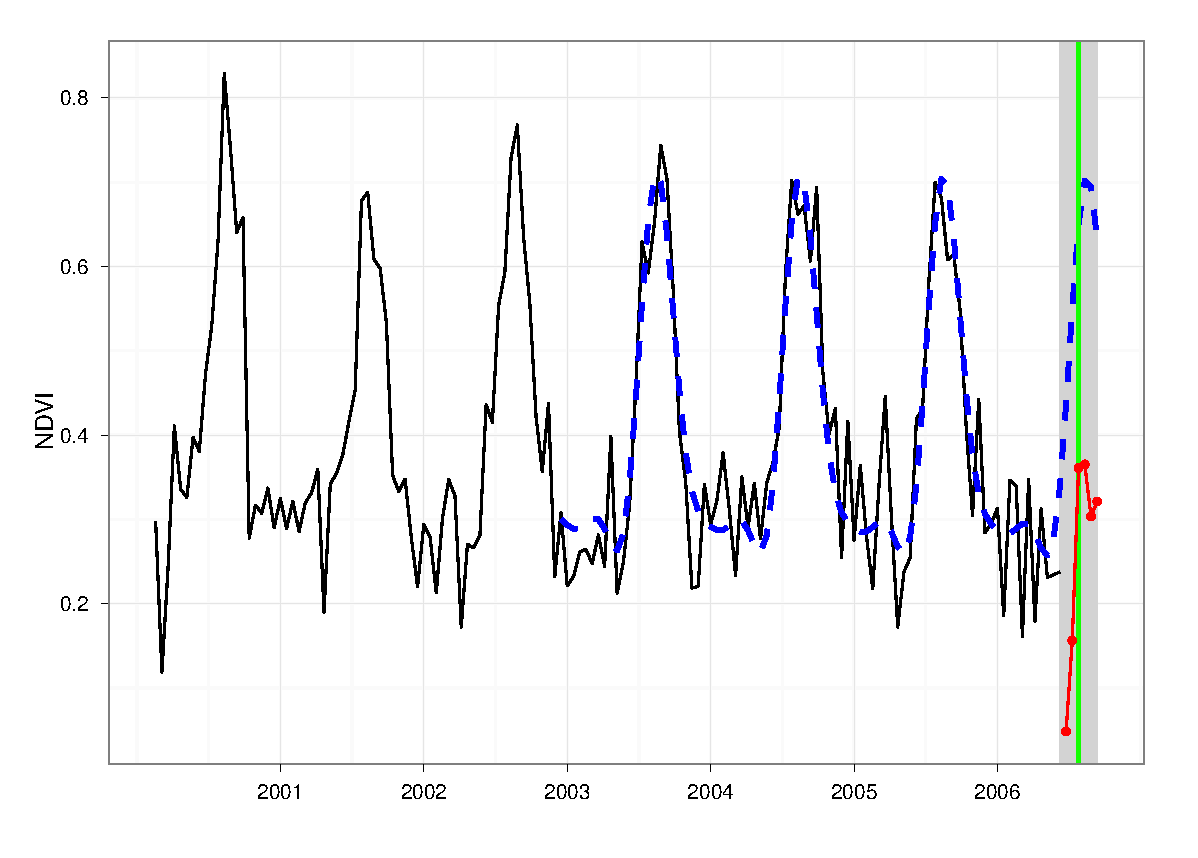
\includegraphics[height=0.5\textwidth]{figs/Sim_Monitoring_ggplot.eps}
  \caption{Simulated 16-day MODIS NDVI time series with $a$ = 0.4, $\sigma$ = 0.05, containing one simulated abrupt change with $m$ = $-$0.3). The period from 2000 until mid 2006 (i.e., the time step just before the simulated break), is considered the \emph{history period} and the period after the simulated break is the \emph{monitoring period} (grey background). The monitoring period contains 6 observations  ($d$ = 6) as shown by the \textcolor{red} {red} line. The result of applying the monitoring approach on the  simulated NDVI series is also shown. A stable history period is identified within the history period (i.e. 2003 until mid 2006) and used to model the normal data variation of the stable history period and predict normal data variation during monitoring period (\textcolor{blue} {blue} dashed line) to enable disturbance detection (Section~\ref{sec:MonStrucChange}).  Here, a disturbance is detected and the estimated time of disturbance is shown by the vertical \textcolor{green} {green} line.}
  \label{fig:SimMonitor}
\end{figure}

\subsection{Spatial application on MODIS 16-day NDVI time series}\label{sec:RealData}

The use of the real-time monitoring approach is demonstrated using MODIS NDVI satellite image time series. We selected the 16-day MODIS NDVI composites with a 5.6~km spatial resolution (MOD13QC1 collection~5), since this product provides frequent information at a global scale that is ideal to detect and study large scale physical, biogenic or anthropogenic disturbances. The MOD13C1 images were acquired from February 2000 to  July 2011 covering Somalia. We used the MODIS quality assurance flags to select only cloud-free data of optimal quality. Moreover, a NDVI time series was only selected for analysis when it lacked less than 15\% of the data \citep{Beurs2009}.
Furthermore, the noise level was estimated to compare the performance of the method with the obtained results from the simulation experiment. The noise level is estimated by deriving the standard deviation of the residuals from the fitted seasonal-trend model (Eq. \ref{eq:lmod}) of the stable history period.

\section{Results and discussion}

\subsection{Simulation experiment}

Fig.~\ref{fig:SimNr} illustrates the probability for detecting a break within the monitoring period of a time series while varying the noise level ($\sigma$), magnitude of simulated disturbance ($m$) and the amount of data available in the monitoring period ($d$). The seasonal amplitude ($a$) did not influence the probability for break detection and results shown in Fig.~\ref{fig:SimNr}  are valid for the different simulated $a$'s (Table~\ref{table:simpar}). The length of the identified stable history period also did not influence the probability for break detection (results not shown).

% noise level
Noise level ($\sigma$), available data in the monitoring period ($d$), and the magnitude ($m$) of the simulated disturbance are the drivers of the capacity to detect disturbances (Fig.~\ref{fig:SimNr}). As such, the probability to detect disturbances can be determined by deriving the noise level  in real time series data of which timing and magnitude of disturbance and available data ($d$) during the disturbance is unknown.

% importance of the simulation experiment
This confirms the importance of a simulation experiment when developing global change detection methods. Novel methods can be tested in a controlled environment while varying individual parameters. When detecting changes in real data at a global scale often accurate field data about disturbances and other influence factors (e.g. quality of the time series observations) are not available. However, it is challenging to create simulated time series that approximate remotely sensed time series, because these contain combined information on vegetation phenology, inter-annual climate variability, disturbance events, sensor conditions (e.g., viewing angle), and signal contamination (e.g., clouds) \citep{Zhang2009}. Therefore, applying the method to real remotely sensed data remains necessary.



% what is not tested here is that when a disturbance occurs later in the monitoring period the probability to detect disturbance is influenced...

% the aim of this method - generic disturbance detection
The method propose here is developed as a fast, generic and globally applicable alert system for disturbances within newly acquired data of available time series derived from in-situ and satellite sensors. We therefore did not assess the accuracy of estimating the time of disturbance. In previous work, the BFAST method was proposed to determine the number, type, and timing of changes within historical time series \citep{Verbesselt2009a} whereas here we specifically focussed on disturbance detection in newly acquired observations. A possible operation workflow for disturbance monitoring could as such be to first verify whether or not a disturbance is occurring using the method proposed here and then second once a disturbance is detected and more data is acquired timing, magnitude and direction of change can be determined.






% important to be discussed - here the seasonality has no influence since the seasonal-trend model is perfectly able to account for the simulated seasonal variation. However, in reality especially in ecosystems with a large inter-yearly variation in seasonality (e.g. late or early start of the growing season) these models have difficulties accounting for these phenological shifts. This, again, illustrates the importance of applying the method to real MODIS data in an area where there is a high probability of inter-yearly variation in seasonality due to unpredictable rainfall patterns (add reference). However, when applying the method in a forested environment we will illustrate that there is often is a small seasonal variation due the saturation of the NDVI signal and deeper rooting systems of forests which makes them more resistant to local climate variability. Here noise levels are smaller and therefore the method will be able to detect smaller disturbances faster (i.e. small detection delay)
% length of the history period... is not been tested here... no disturbances have been simulated in the history period since the method is developed a rough method for stability estimation.

% explain the noise level - which actually does simulate the effects of seasonal variability which often ends up beiing noise!!! (this also links to the phenological change detection proposed in previous remote sensing of environment paper.

% to do search for a forest in Somalia - i.e. high median NDVI - in order to illustrate this concept - when can also illustrate this for a pixel modis MOD13C1 for a fire in Victoria (coordinates -> query from the database - and plot an example).

% the delay time for disturbance detection is important!!! (how fast can a change be detected?)
% where does it work and what needs to be done to implement the method?

Furthermore, Fig.~\ref{fig:SimNr} shows that a break with $m = -0.2$ can be detected when noise level ($\sigma$) is smaller than 0.04 and $d = 3$ (i.e., 3 images available).  When the magnitude of the break is larger (e.g., $m = -0.3$), less data points ($d<3$) are required in the monitoring period for a similar amount of noise (e.g., $\sigma < 0.04$) in the history period. 


\subsection{Spatial application on MODIS 16-day NDVI time series}

While the data and methods used here are appropriate for proof-of-concept development \citep{White2006}, other applications (e.g., deforestation monitoring in tropical forests or oil spill detection) will mandate further calibration and validation.


The main purpose of applying the real-time monitoring approach to MODIS 16-day NDVI time series is to illustrate a proof-of-concept of real-time monitoring for forest areas. Fig.~\ref{fig:SpatNoise} shows the spatial variation of the noise level ($\sigma$) in the study area. The lower noise levels correspond to the forested area within the boundaries of the Pinus radiata plantation. Higher noise levels occur outside the plantation area and correspond to the different grassland types as shown in \citet{Verbesselt:2010wo}. Higher noise levels in grasslands are caused by a large seasonal NDVI amplitude and inter-annual phenological shifts (e.g., shifts in the start and end of the growing season) due rainfall and temperature dynamics.

Therefore, results in Fig.~\ref{fig:SpatTimeofChange} and Fig.~\ref{fig:SpatLStableHist} are shown for the region within the boundaries of the forest plantation, which approximately corresponds to the lower noise levels in Fig.~\ref{fig:SpatNoise} and the noise range used in the simulation experiment illustrated in Fig.~\ref{fig:SimNr} (Table~\ref{table:simpar}).
%Grassland are influenced more by rainfall and temperature dynamics causing a high seasonal amplitude and large phenological shifts (e.g., start and end of the growing season) \citep{Verbesselt:2010wo}, which explains the higher noise levels. 
% remove data where the lenght of season is smaller then 1.5 years?
Fig.~\ref{fig:SpatTimeofChange} illustrates the time of the detected changes in 2006. Many changes are detected in 2006 due to a drought that occurred around that time in combination with ongoing harvest operations. Fig.~\ref{fig:SpatLStableHist} shows the length of the stable history period and illustrates where and when changes occurred in the history period (e.g., a recent harvest operation). Results shown in Fig.~\ref{fig:SpatTimeofChange} and~\ref{fig:SpatLStableHist} are illustrated for three locations within the study area in Fig.~\ref{fig:realmonitoring} and~\ref{fig:shorthistory}.

Fig.~\ref{fig:realmonitoring} and~\ref{fig:shorthistory} are examples for specific locations in the study area illustrating the detected (1) disturbance and (2) the identified length of the stable history period. First, drought stress in 2006 is the main driver of the disturbance detected in the top graph of Fig.~\ref{fig:realmonitoring}, whereas a harvest operations explains the change detected in the bottom graph of Fig.~\ref{fig:realmonitoring}. Second, a different length of the automatically identified stable history is also visible in Fig.~\ref{fig:realmonitoring} (top versus bottom). A larger impact of a drought period in 2003 on the NDVI time series of a Pinus radiata plantation (top versus bottom graph) could explain the shorter stable history period. Fig.~\ref{fig:shorthistory} illustrates an ongoing harvests operation during the history period which explains the shorter identified stable history period. Nonetheless a change is still detected in 2006 due the ongoing effects of the harvest operation.

% add age of the plantations to the results the explain results better.


\section{Discussion and further work}

% discuss the effect of the temporal resolution of the data
 
% compare our method with the disturbance detection algorithm of Potter2003!!! Discuss. Have a look at Potters results.

% discuss that the stable history period detection is a rough measure for stability assessment - and can be further improved to be more sensitive to seasonal changes e.g. by combining different score based function instead of just one, the MOSUM criteria applied here. % the objective of the paper here is to propose, assess, and demonstrate a novel approach for global disturbance assessment. Further improvement is possibles and we recommend especially further field data based validation in case the method is applied to detect specific disturbances.




% tested and demonstrated for forested areas further testing is required for areas with large seasonal amplitudes.
% magnitude of change can also be derived from the model... but was not done in this study.

\begin{enumerate}[(1)]

\item  Further testing is required to assess the impact of phenological shifts (e.g., changes in the start/end-of-season) on the real-time monitoring approach. We demonstrated the monitoring approach for NDVI time series derived from forested areas where seasonal NDVI amplitude and the impact of phenological shifts are relatively small when compared to grassland areas, for example. Continuous modelling of the seasonality using the proposed real-time concept and seasonal-trend model allows for relating remote sensing to a continual process of land surface phenology change instead of a single date extraction \citep{Verbesselt:2010wo,White2006}.  Grasslands, for example, demonstrate large inter-yearly seasonal variation caused by a early or late start/end of the growing season which is more difficult to be fitted within multi-year time series data. This is illustrated by the higher noise levels (i.e., standard deviation of the residuals of the season-trend model used in this study) in the grasslands surrounding the forest plantations. Further testing is required for areas with a dominant herbaceous vegetation layer (e.g., grasslands, agriculture, and savannah areas). The proposed concept, however, has the potential to detect phenological shifts in near-real time \citep{Verbesselt:2010wo} but still need to tested.
The real-time monitoring approach is validated and tested for forested areas. It can be implemented in an operational framework for deforestation monitoring such as, the Brazilian real-time deforestation monitoring system \citep[DETER,][]{Shimabukuro:2006vb} or \citep[CLASLITE,][]{Asner:2009wa} and as an alert system in other regions in the world (e.g., Indonesia, Vietnam) where a real-time monitoring system is not implemented yet but deforestation is occurring at a fast rate \citep{Asner:2011fa}. 

% search for extra real-time monitoring projects/add more references. GLASLITE

\item Further work is needed to explore the use of the identified stable history period when implementing the method within an operation framework. The length of the stable history is identified for modelling normal, stable data variation within the history period to enable differentiation from abnormal changes in the monitoring period. The method for identifying the stable history is based on the structural change detection methods \citep{Bai2003,Zeileis:2010tt} and is implemented to assess stability of the history period. The method is a basic and fast approach with the objective of verifying whether or not a structural change is occurring while stepwise going back in history. It is not implemented to determine accurately the time of change but for testing whether of not a change is occurring in the history period \citep{Zeileis2002}. The BFAST approach is developed to detect and characterise accurately the time and magnitude of change within time series \citep{Verbesselt2009a}. The approach to asses the stability of the history period can be used e.g., for identifying when and where in recent history disturbances occurred or to restrict detection of changes in the monitoring period to time series which have a stable history period e.g., longer than 2 years. Alternatively, a stable history with a fixed length can also be used based on expert knowlegde but is not recommended for regional or global scale analysis due to a loss in flexibility. In summary, the length of the stable history as such can be used to optimise the real-time change detection approach depending on the objectives of operational real-time disturbance system.

\item The real-time monitoring could be further improved by; (a)~including other explanatory variables in the monitoring model (e.g., temperature, rainfall)
which will contribute to model the data and determine what is normal versus what is abnormal (GAM modelling references), (b)~determining the magnitude of
change from the fitted parameters of seasonal-trend model similar as implemented in the BFAST approach \citep{Verbesselt2009a} and (c)~the monitoring model proposed here can also be used as a forecasting model. Similar to current real-time monitoring approach, forecasting requires a profound understanding of vegetation dynamics and vegetation interaction with the atmosphere, combined with proper data analysis techniques  \citep{LeiJi:2004kx}.

\item To be included in the above paragraph: Climate tipping points etc. might be an nice reference \citep{Lenton:2011ke} and illustration of current ideas and potential use of 

\end{enumerate}

\readme{Achim could you double check whether I formulate the 2nd paragraph correctly.}

\section{Conclusion}

Results of the simulation experiment and application on 16-day MODIS NDVI time series illustrate a proof-of-concept of the proposed time series based
real-time monitoring approach. The change detection approach is a generic, data driven approach based on statistical principles applicable to different
types of time series (e.g., in-situ or satellite sensors). The method can be applied to time series with a higher temporal resolution (e.g., hourly, daily
or 8-day time series) to enable rapid response to detected disturbances. Application of the  proposed method to the MODIS rapid response data (e.g., \url{http://lance.nasa.gov/}) or data available from geostationary satellites (e.g., \url{http://www.cmsaf.eu/}) can enable fast and automated detection of disturbances. 


Currently, real-time satellite images and their derivatives are routinely produced and published on the World wide Web (e.g., \url{http://rapidfire.sci.gsfc.nasa.gov/} or \url{http://www.dmcii.com/index.html}) but methods for real-time monitoring and change detection are lacking. Here, we proposed a time series based real-time monitoring approach that enables the detection of changes within newly acquired images or data.
The real-time monitoring approach is a generic data driven approach that can be applied to any type of time series data. Results from the simulation experiment demonstrated that the noise level within the time series together with the amount of data available in the monitoring period are the main drivers of the capacity to detect disturbances within newly acquired images. Results from the simulation experiment are also applicable for time series with a higher temporal resolution as noise level will also be a driver in these time series (e.g., daily).
The simulation experiment and application on MODIS 16-day data was focussed on testing the method for detecting changes in forested areas. Further work is require to test and optimise the method for ecosystems with a dominant herbaceous cover (e.g., grassland, agriculture) .

%Land cover types with a dominant herbaceous cover have a high seasonal amplitude together with large inter-yearly phenological shifts.

The method has the following characteristics that make it appropriate for real-time change detection implementation at different spatial scales. The method
(1)~is fast and require a minimum a mount of processing time (e.g., 0.04 seconds to analyse 6 year long 16-day time series  on a normal desktop computer),
(2)~does not require the definition of thresholds, change type or even minimum amount of data as required by the BFAST approach, (3)~can analyse time series
with data gaps (e.g., masked clouds or sensor defects) and does not require gap filling techniques, and 4) it analyses the full temporal detail of a time
series and it not restricted to definition and time dependent phenological metrics. Furthermore, the real-time monitoring method is implement in open-source
software environment and is freely available on \url{http://bfast.R-Forge.R-project.org/} . The methods are available in the \emph{bfast} package for {R} \citep{R}
from \url{http://CRAN.R-project.org/package=bfast}.


The method described in this study is available in the \emph{bfast} package for {R} \citep{R} from the Comprehensive
{R} Archive Network (CRAN) at \url{http://CRAN.R-project.org/package=bfast}.
It can be used for disturbance detection within other data sets (e.g. temperature, rainfall, $CO_2$ time series data) or be integrated within monitoring
frameworks (e.g., \url{http://rapidfire.sci.gsfc.nasa.gov/}), and used as an alarm system to provide information on when and where
significant disturbances occur. 



%This validation approach by combining tests with simulated and real data should be a standard practice when validating novel change detection approaches. Furthermore, methods being proposed should also be made available to other scientist enabling the reproducibility of the research and collaboration towards further improvement of the methods.



%The approach is adaptable to different remote sensing technologies and provides a foundation for ascribing a sequence of ground conditions (e.g., snowmelt, vegetative growth, pollen production, insect phenology) to remotely sensed land surface phenology observations \citep{White2006}.

%Deviations from �normal� land surface phenological development can be the first indications of important changes in forest health, including disturbance and recovery, carbon status, and even climatic shifts.

\section{Acknowledgements}

This work was undertaken using expertise and field data available via the program of the Cooperative Research Center for Forestry: Monitoring and Measuring (\url{http://www.crcforestry.com.au}). This work was funded by a Marie-Curie IRG fellowship within the European Community's Seventh Framework Program to Jan Verbesselt (grant agreement $268423$). Thanks to Darius Culvenor and Glenn Newnham whose comments greatly improved this paper. We greatly appreciate the constructive feedback we have received from the x reviewers.


\bibliographystyle{model5-names}
\bibliography{refs}

\newpage

\section*{Figures}

 (For interpretation of the references to color in this figure legend, the reader is referred to the web
 version of this article.)

\begin{figure}[htp]
\centering
    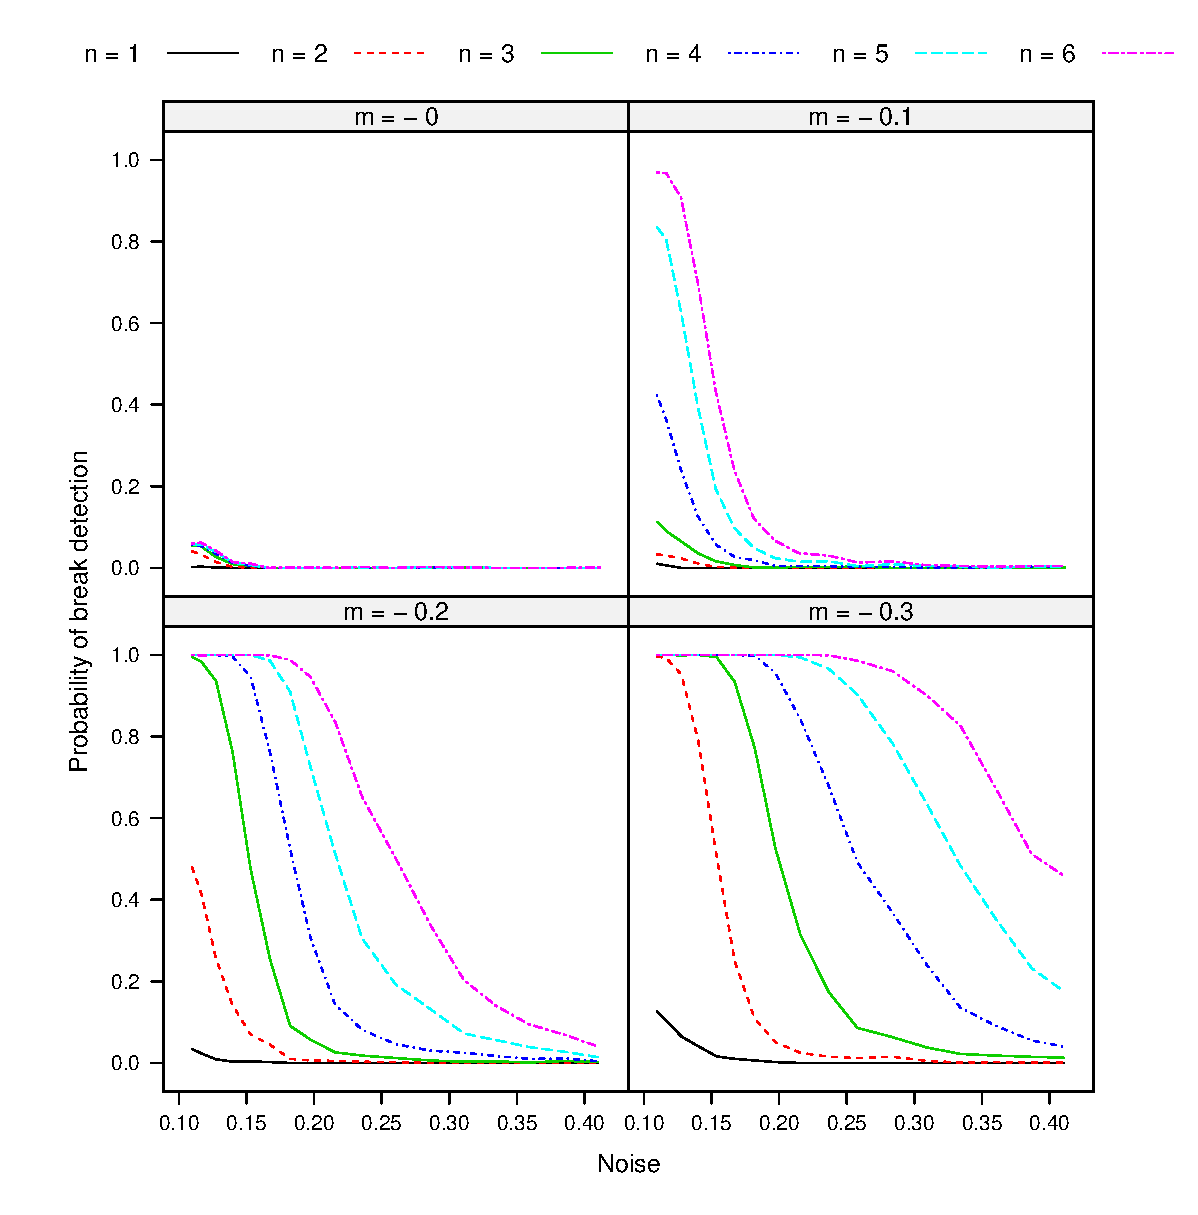
\includegraphics[height=0.9\textwidth]{figs/NrDetections_Time_1000.eps}
  \caption{Results from the simulation experiment (1000 iterations) illustrating the probability for break detection in the monitoring period while varying the amount of noise ($\sigma$), magnitude of the simulated break ($m$), and amount of data  available in the monitoring period ($n$). The units of the x and y-axis are noise (i.e., $\sigma$ NDVI of the residuals of the fitted seasonal-trend model on the history period) and probability of detecting a break (i.e., proportion of detected breaks in 1000 iterations). See description of the simulation experiment for more details (Section \ref{sec:Valsim}). }
  \label{fig:SimNr}
\end{figure}

%\begin{figure}[htp]
%\centering
%    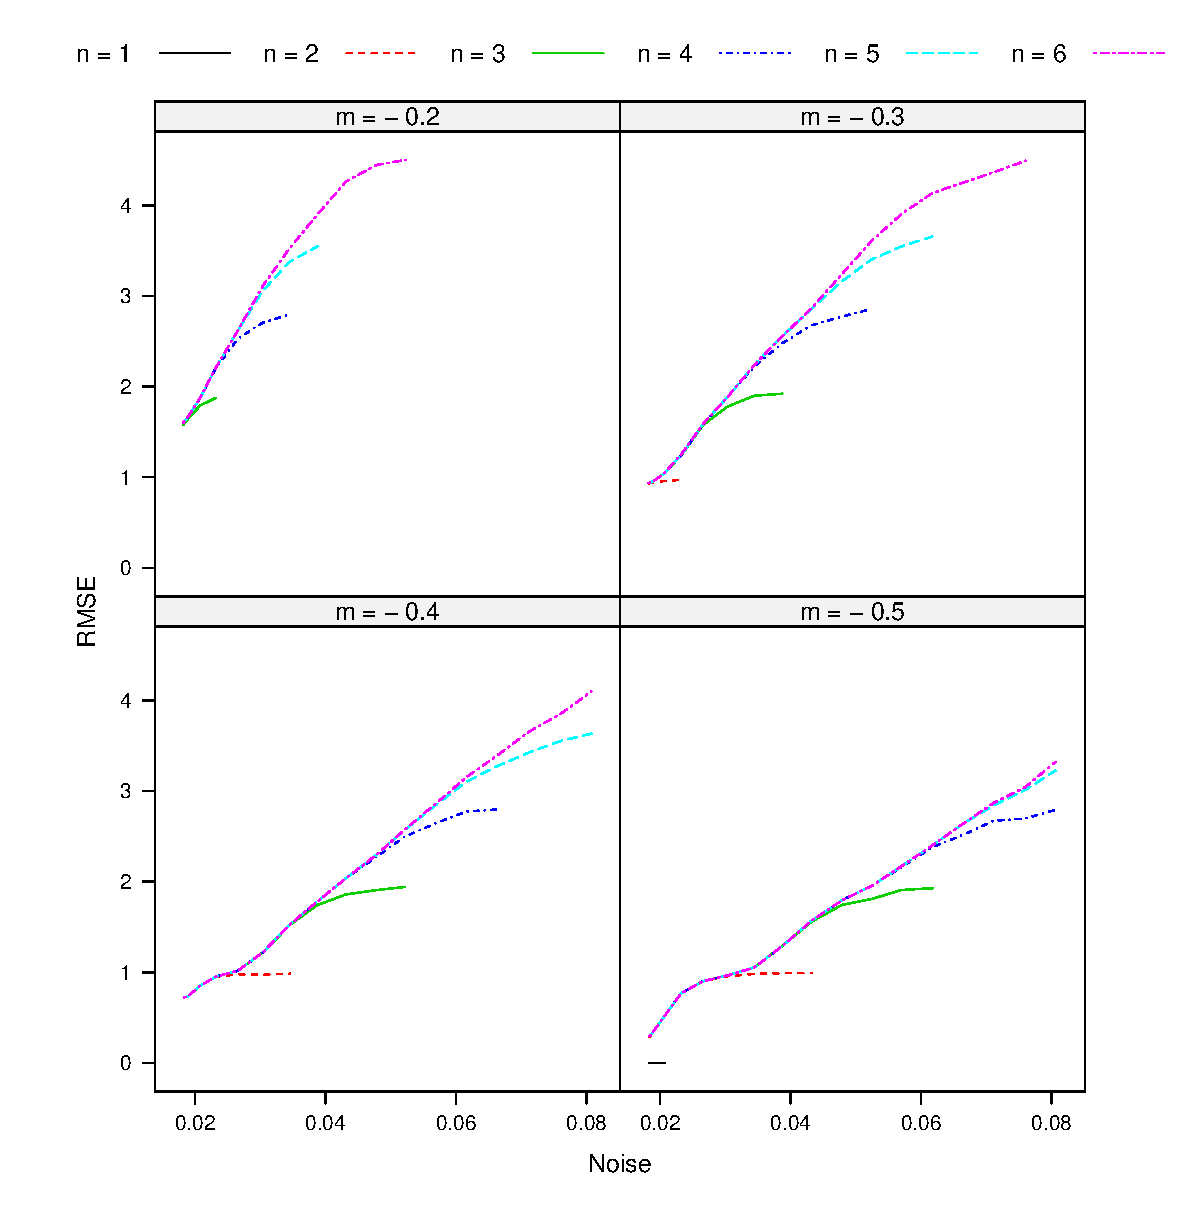
\includegraphics[height=0.9\textwidth]{figs/RMSE_Time_1000.eps}
%  \caption{Results from the simulation experiment (1000 iterations) illustrating the accuracy of time estimation of the detected breaks while varying the amount of noise, magnitude of simulated break ($m$), and amount of data available in the monitoring period ($n$). The units of the x and y-axis are noise (i.e., noise range expressed in NDVI) and RMSE (i.e., time steps between images where 1 equals a 16-day period). See description of the simulation experiment for more details (Section \ref{sec:Valsim}).}
%  \label{fig:SimRMSE}
%\end{figure}

%\begin{figure}[htp]
%\centering
%    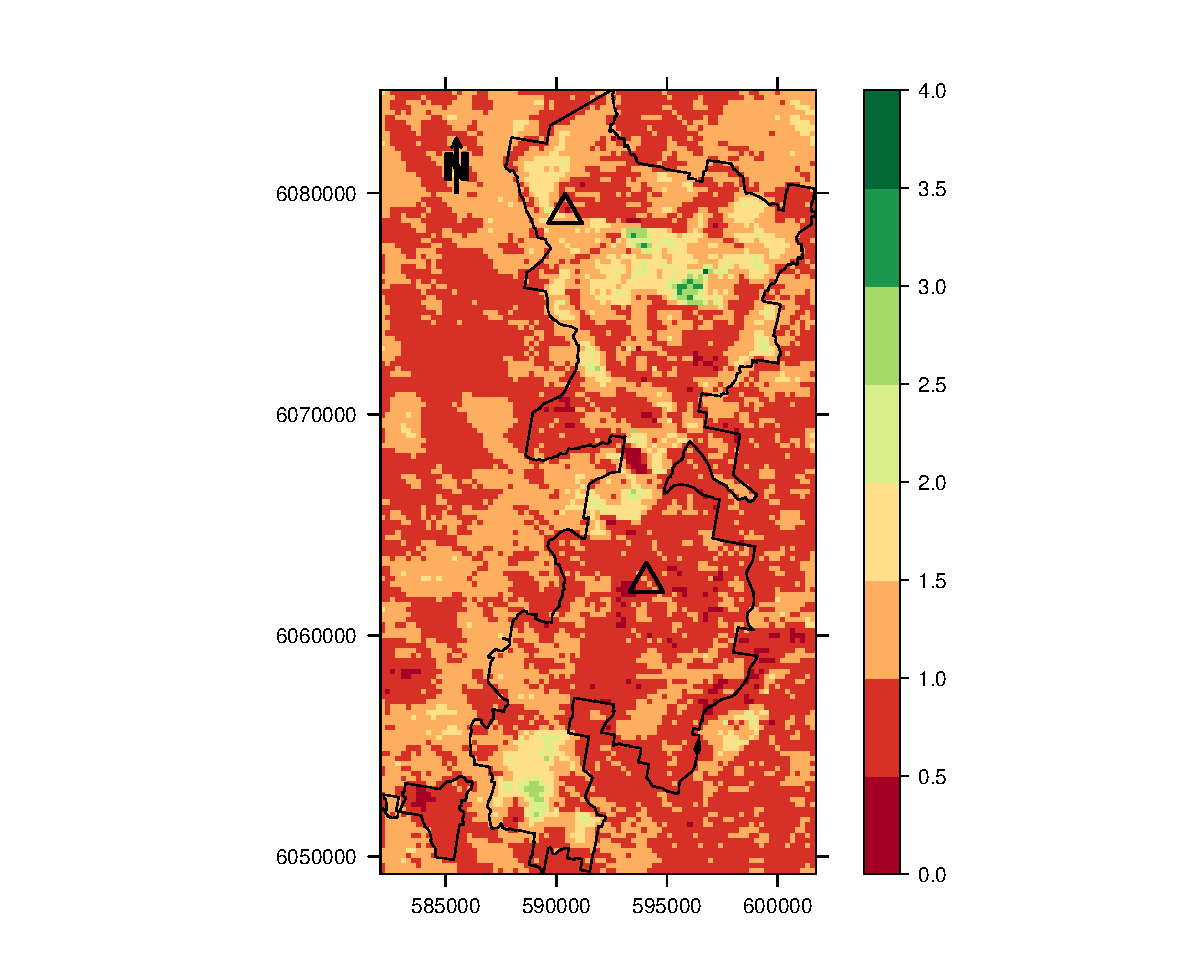
\includegraphics[height=0.9\textwidth]{figs/SignaltoNoiseRatio.eps}
%  \caption{Spatial variation of the signal to noise ratio is the study area. (Try out: only for your information - not sure whether I will include this in the paper) }
%  \label{fig:SpatSignalNoise}
%\end{figure}

\begin{figure}[htp]
\centering
    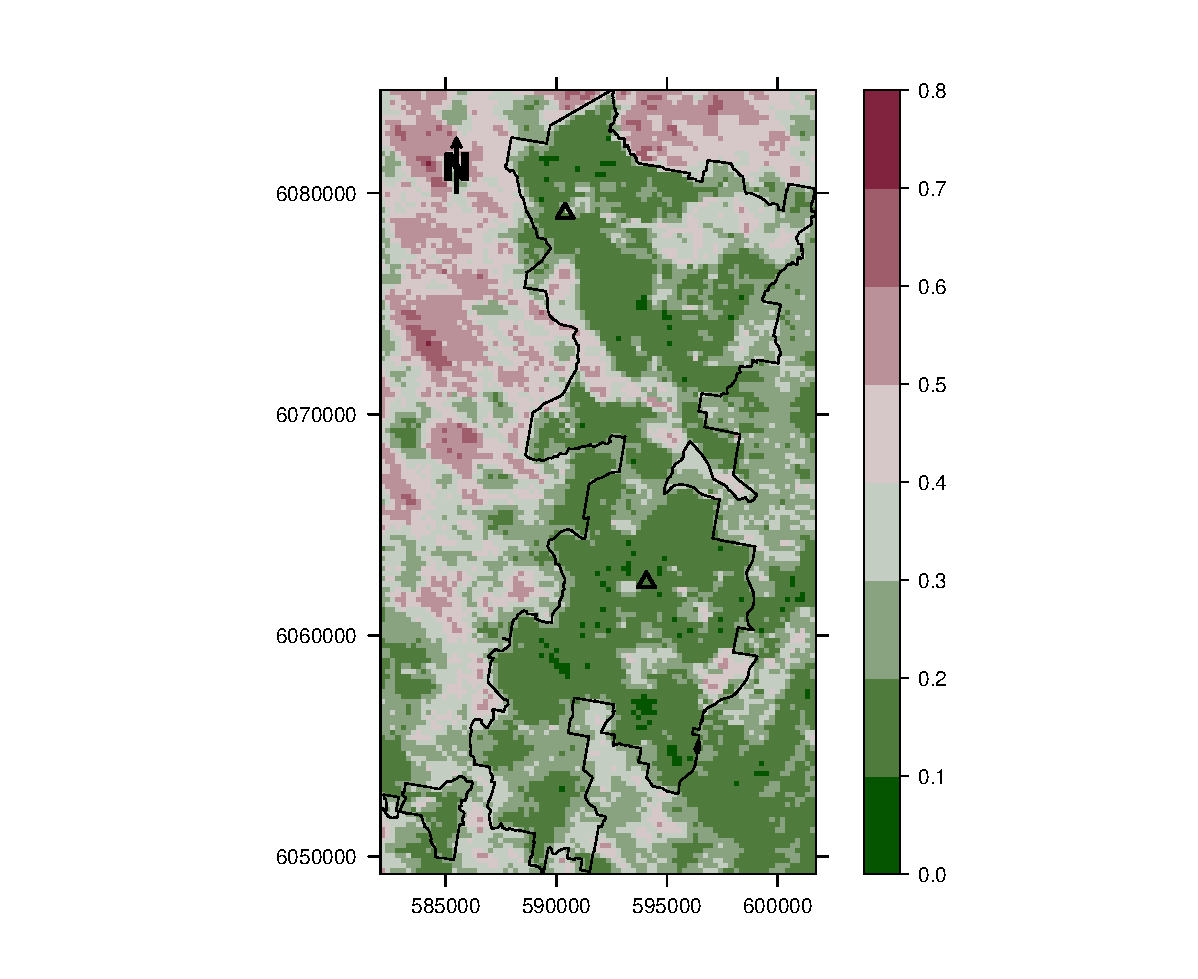
\includegraphics[height=0.9\textwidth]{figs/Noise.eps}
  \caption{Spatial variation of the noise level (i.e., the standard deviation of the residuals of the stable history model) in the study area, a forested area in south eastern Australia. The black line indicates the boundary of the Pinus radiata plantation, which corresponds to the area with a lower noise level. The plantation is surrounded by grasslands. Examples of real-time change analysis for three locations ($\triangle,+$~and~$\diamondsuit$) are shown in Fig.~\ref{fig:realmonitoring} and \ref{fig:shorthistory}. }
  \label{fig:SpatNoise}
\end{figure}

\begin{figure}[htp]
\centering
    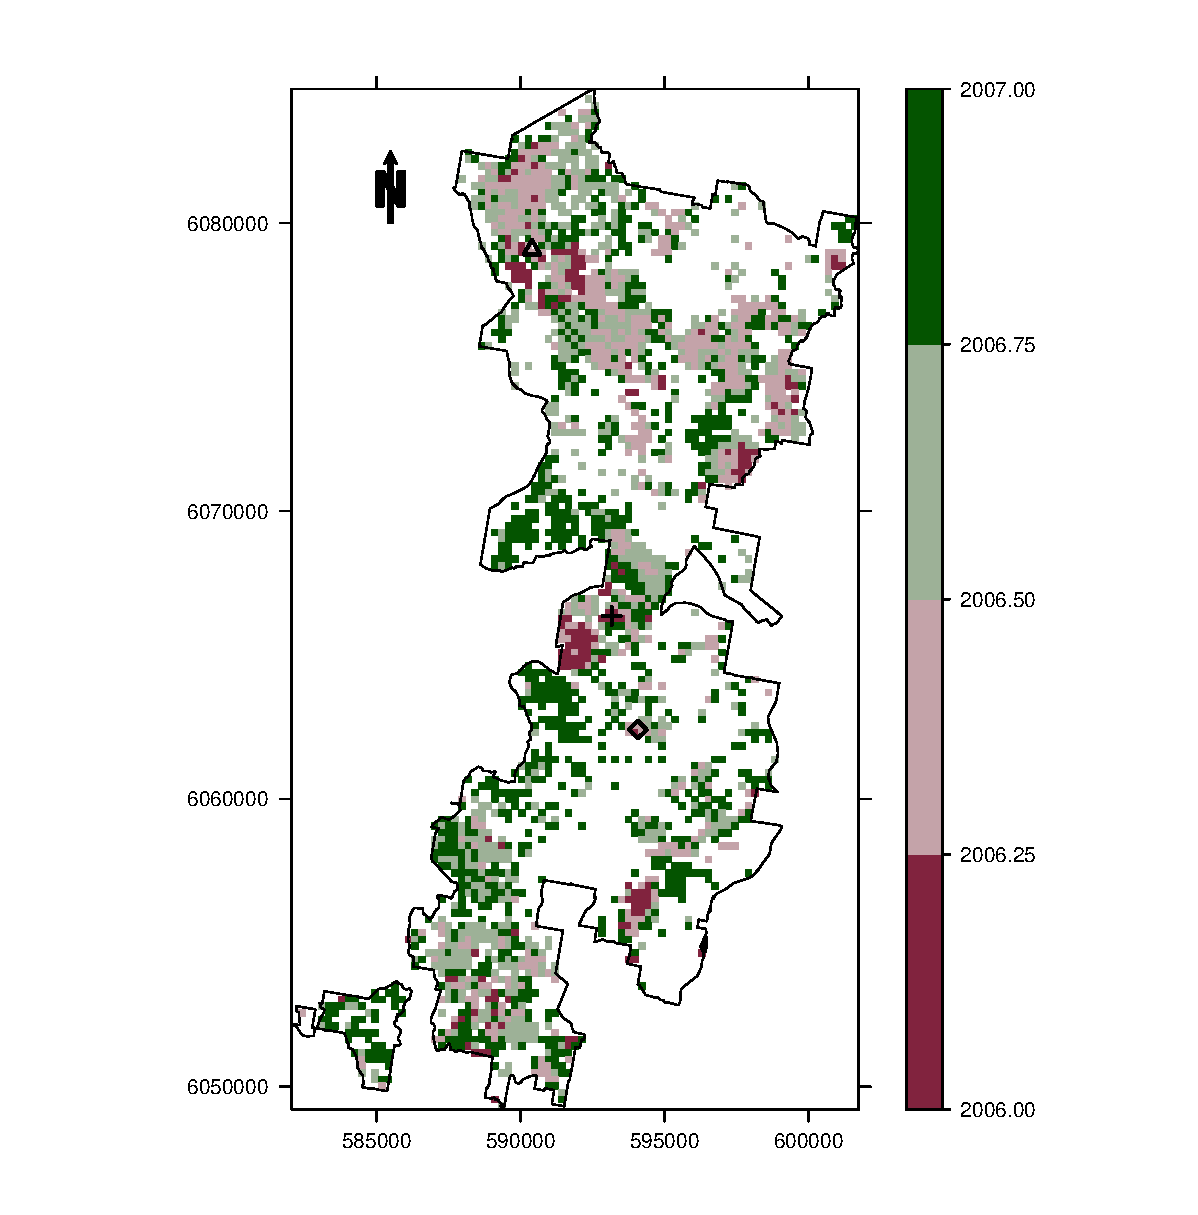
\includegraphics[height=0.9\textwidth]{figs/TimeofChangein2006_II.eps}
  \caption{Time of detected changes within the study area in the monitoring period (i.e., 2006), where white indicates that no change is detected for a forested area in south eastern Australia. The black line indicates the boundary of the Pinus radiata plantation which is surrounded by grasslands. Examples of real-time change analysis for three locations ($\triangle,+$~and~$\diamondsuit$) are shown in Fig.~\ref{fig:realmonitoring} and \ref{fig:shorthistory}. }
  \label{fig:SpatTimeofChange}
\end{figure}

\begin{figure}[htp]
\centering
    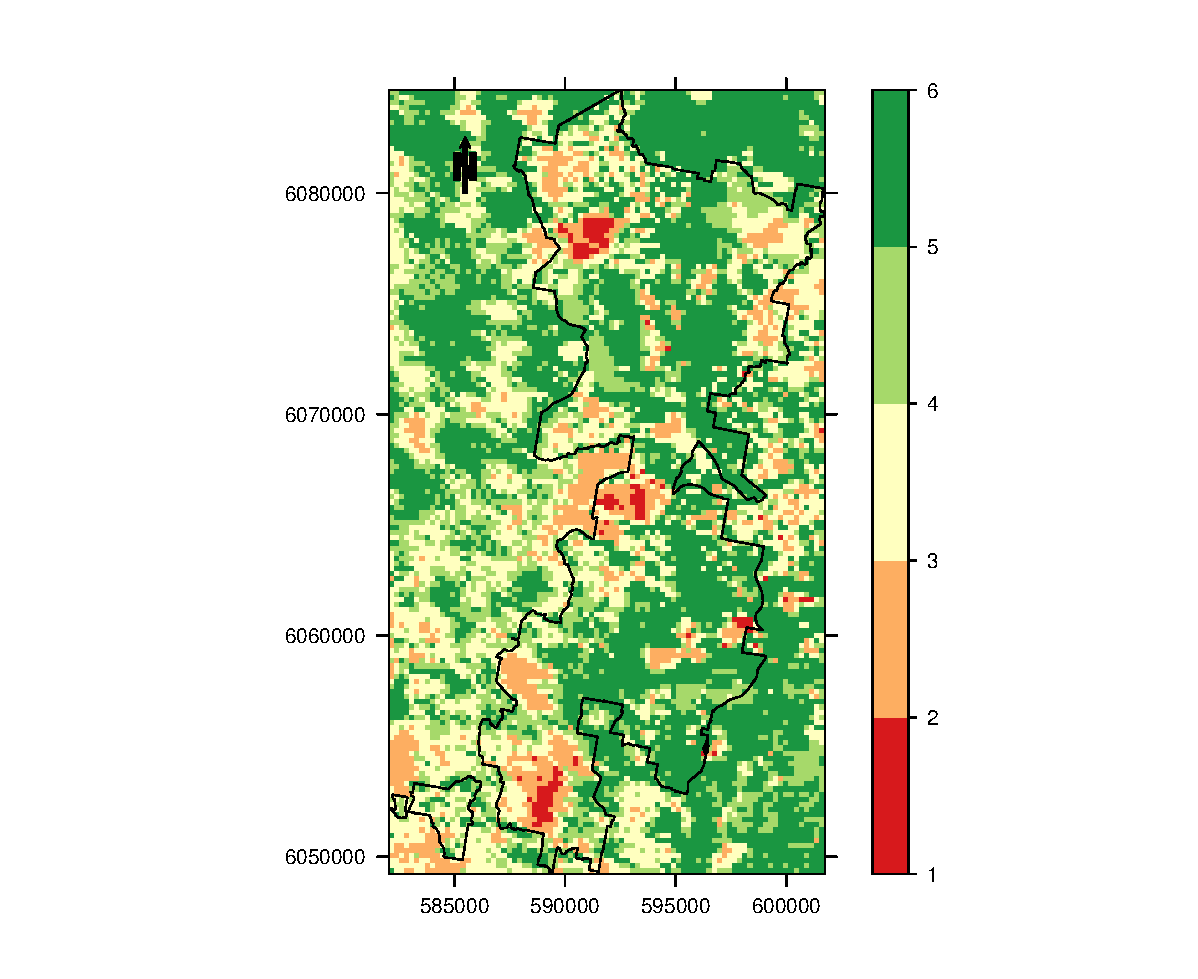
\includegraphics[height=0.9\textwidth]{figs/LengthStableHistory.eps}
  \caption{Spatial variation of the length the stable history period (expressed in years, i.e., 23 16-day images) of a forested area in south eastern Australia. The black line indicates the boundary of the Pinus radiata plantation, which is surrounded by grasslands. The length of the history period indicates when in the history period a potential disturbance occurred (e.g., shorter length indicates a more recent disturbance). Examples of real-time change analysis for three locations ($\triangle,+$~and~$\diamondsuit$) are shown in Fig.~\ref{fig:realmonitoring} and \ref{fig:shorthistory}.}
  \label{fig:SpatLStableHist}
\end{figure}

\begin{figure}[htp]
\centering
    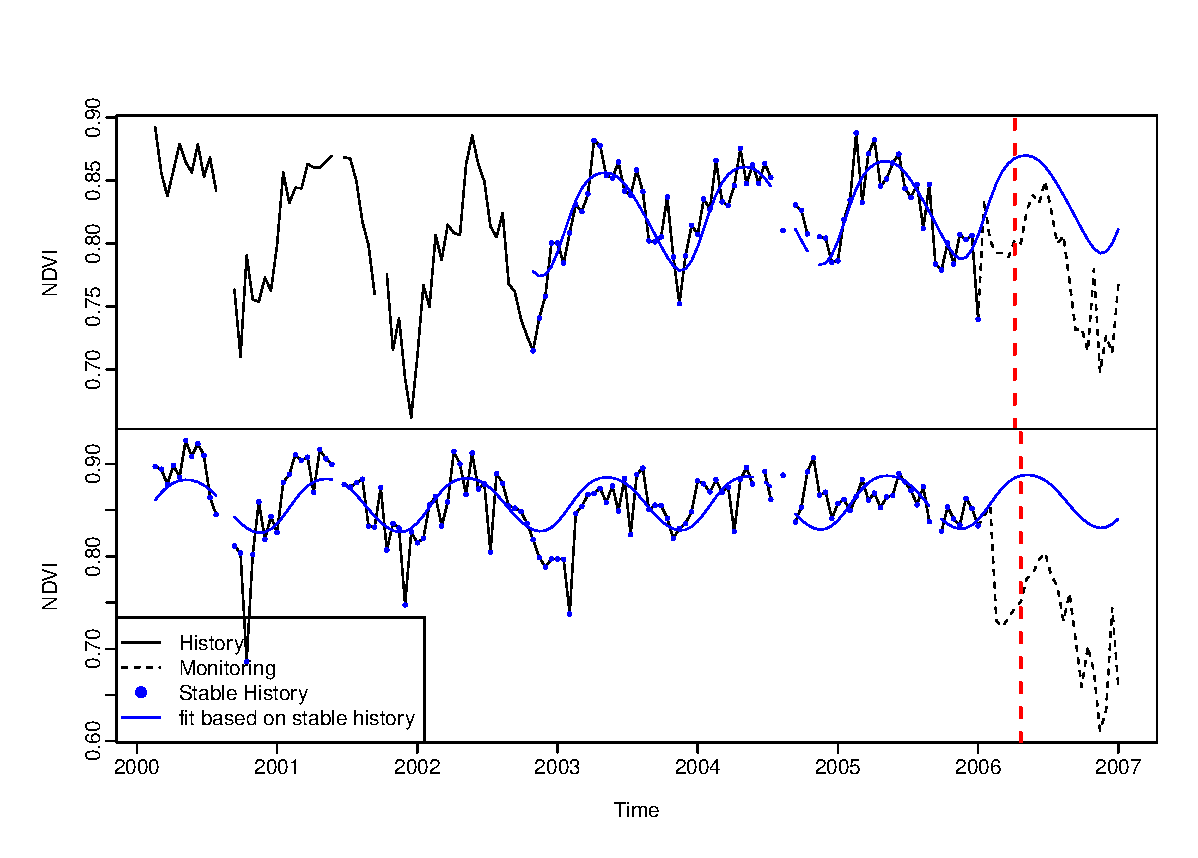
\includegraphics[height=0.6\textwidth]{figs/realmonitoring.eps}
  \caption{
  %plot 120 and 8
  Results of real-time monitoring approach applied to 16-day MODIS NDVI time series for two locations, i.e., $\diamondsuit$ (top) and $\triangle$ (bottom) on Fig.~\ref{fig:SpatNoise}, \ref{fig:SpatTimeofChange} and \ref{fig:SpatLStableHist}), situated within the Green Hills study area. In both time series a break (vertical red dashed line in 2006) is detected in the monitoring period (i.e., 2006) while using 2000 until end of 2005 as a history period. A stable history period (blue dots) is automatically detected with the history period. The method is able to deal with time series with data gaps (e.g., after cloud removal) which is illustrated by data gaps within the data analysed and model fit based on the stable history period.}
  \label{fig:realmonitoring}
\end{figure}

\begin{figure}[htp]
\centering
    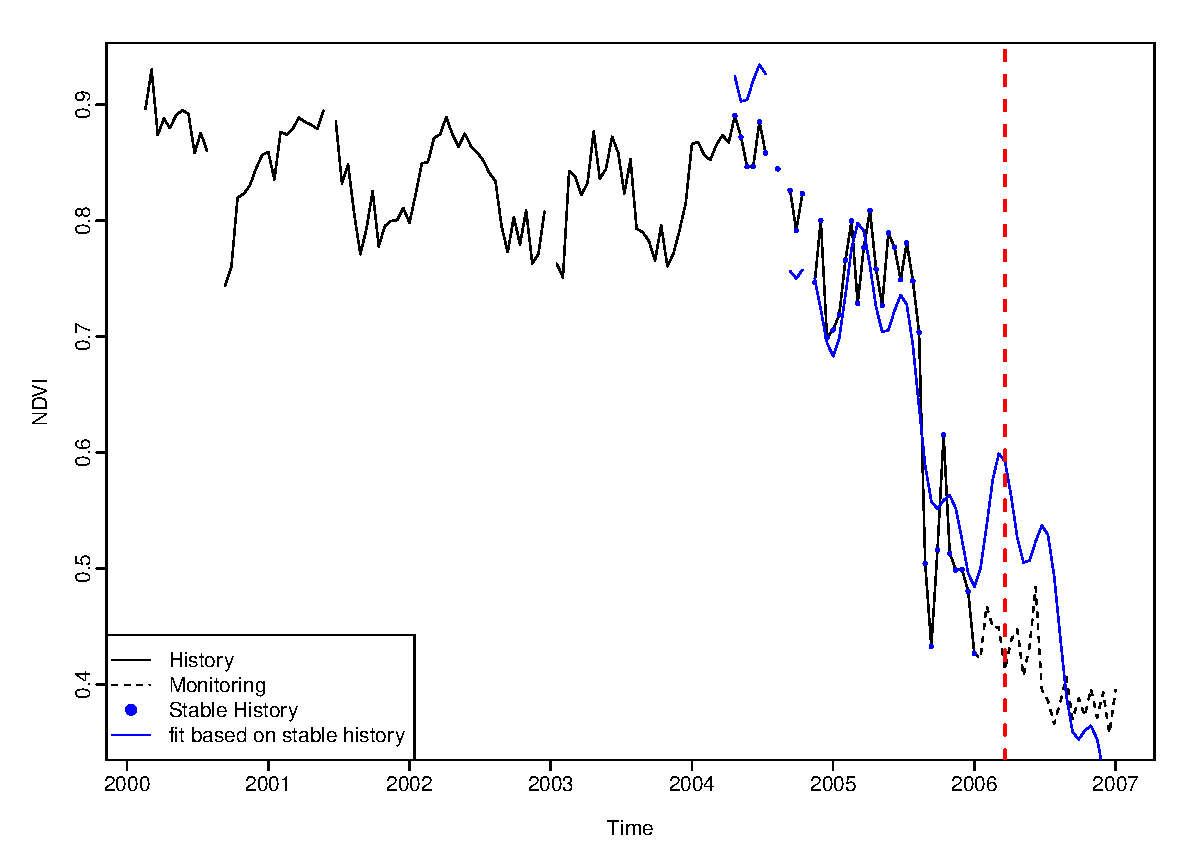
\includegraphics[height=0.6\textwidth]{figs/shorthistoryperiod.eps}
  \caption{
  Results of real-time monitoring approach applied to 16-day MODIS NDVI time series for a location situated within the Green Hills study area (i.e., the $+$ symbol on Fig.~\ref{fig:SpatNoise}, \ref{fig:SpatTimeofChange} and \ref{fig:SpatLStableHist}). A break (vertical red dashed line in 2006) is detected in the monitoring period (i.e., 2006) while using 2000 until end of 2005 as a history period. A short stable history period (blue dots) is detected within the history period due to an ongoing harvest operation from 2005 onwards. The method is able to deal with time series with data gaps (e.g., after cloud removal) which is illustrated by data gaps within the data analysed and model fit based on the stable history period.}
  \label{fig:shorthistory}
\end{figure}

%\begin{figure}[htp]
%\centering
%    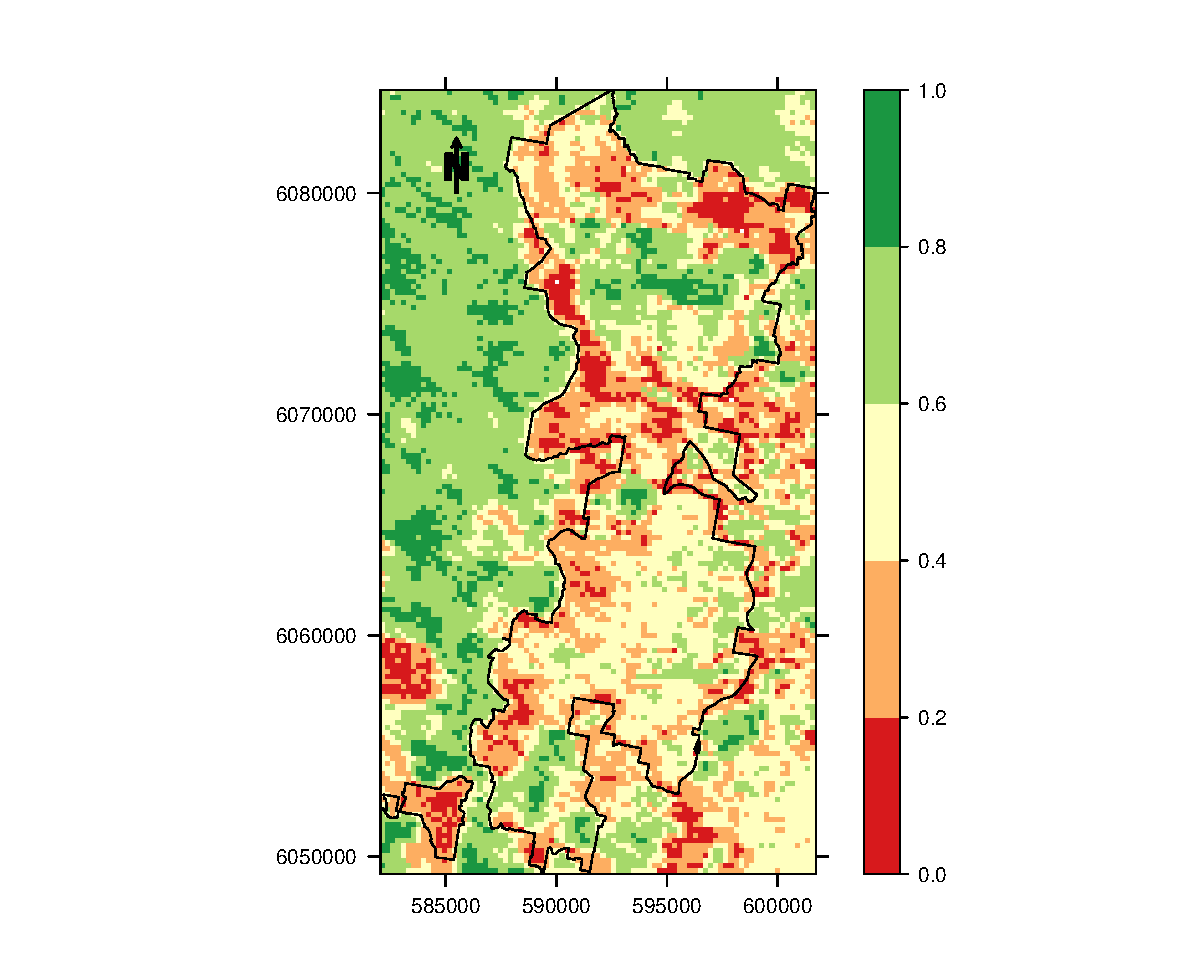
\includegraphics[height=0.9\textwidth]{figs/R2ofthemodelfit.eps}
%  \caption{ Spatial variation of the $R^2$ of the model fit which also depend on the length the stable history period}
%  \label{fig:SpateR2}
%\end{figure}

\end{document}

